View demo code of this section: \democode{02}{2.3}

\subsubsection{Quantum Gates}
In the realm of quantum computing, a quantum gate is a fundamental unit of operation that acts upon qubits, the basic units of quantum information. Just as classical computers use logic gates to manipulate bits of information, quantum computers use quantum gates to manipulate qubits. However, due to the unique nature of quantum mechanics, quantum gates have some distinctive properties.

A quantum gate is essentially a quantum operation that transforms the quantum state of one or more qubits. This transformation is represented mathematically by a unitary matrix, which preserves the quantum state's normalization and reversibility. Unlike classical logic gates, all quantum gates are reversible, meaning it's possible to determine the initial state of the qubits from the final state.

Quantum gates play a pivotal role in the construction of quantum circuits. They allow for the implementation of quantum algorithms by manipulating the quantum states of the qubits in a controlled manner. Quantum gates can perform various operations such as rotations, flips, and entanglement creation, all of which contribute to the unique computational capabilities of quantum computers.

Depending on the number of qubits involved, quantum gates are classified as single-qubit gates or multi-qubit gates. Single-qubit gates operate on individual qubits and are responsible for modifying their states. Multi-qubit gates, on the other hand, perform operations that involve interactions between multiple qubits, enabling the creation of entanglement and more complex quantum operations.

Furthermore, quantum gates can be categorized based on whether they require parameters for their operation. Gates that don't require parameters are known as Non-parameter Gates, while those that do are referred to as Parameter Gates. These gates with parameters provide additional flexibility in quantum algorithms and computations. In \MindQuantum, we can easily construct non-parameterized gate, such as \X, \Y, \Z\ and \H, and parameterized gate, such as \RX, \RY\ and \RZ, with the help or \ParameterResolver.

In essence, quantum gates are the building blocks of quantum computing, allowing for the manipulation, transformation, and interaction of qubits that underpin the unique and powerful computational capabilities of quantum computers.

\subsubsection{Fixed Quantum Gate}
Similar to logic gates in classical circuits, the transition of a quantum circuit state can be achieved through quantum gates. Any quantum gate can be represented by a matrix, the only limitation being that its matrix representation U is a unitary matrix, i.e. ${UU^{\dagger}=I}$.
At the same time, any unitary matrix can define a valid quantum gate, and the dimension of the matrix depends on the number of qubits it operates on.

Here are some examples of single qubit gates, let $\ket{\phi}=a\ket{0}+b\ket{1}$:
\begin{align*}
    I\ket{\phi} & =
    \begin{bmatrix}
        1 &  & 0 \\
        0 &  & 1
    \end{bmatrix}
    \begin{bmatrix}
        a \\
        b
    \end{bmatrix}=
    \begin{bmatrix}
        a \\
        b
    \end{bmatrix}  \\
    X\ket{\phi} & =
    \begin{bmatrix}
        0 &  & 1 \\
        1 &  & 0
    \end{bmatrix}
    \begin{bmatrix}
        a \\
        b
    \end{bmatrix}=
    \begin{bmatrix}
        b \\
        a
    \end{bmatrix}  \\
    Y\ket{\phi} & =
    \begin{bmatrix}
        0 &  & -i \\
        i &  & 0
    \end{bmatrix}
    \begin{bmatrix}
        a \\
        b
    \end{bmatrix}=
    \begin{bmatrix}
        -bi \\
        ai
    \end{bmatrix}  \\
    Z\ket{\phi} & =
    \begin{bmatrix}
        1 &  & 0 \\
        0 &  & -
    \end{bmatrix}
    \begin{bmatrix}
        a \\
        b
    \end{bmatrix}=
    \begin{bmatrix}
        a \\
        -b
    \end{bmatrix} \\
    H\ket{\phi} & =
    \frac{1}{\sqrt{2}}
    \begin{bmatrix}
        1 &  & 1  \\
        1 &  & -1
    \end{bmatrix}
    \begin{bmatrix}
        a \\
        b
    \end{bmatrix}=
    \frac{1}{\sqrt{2}}
    \begin{bmatrix}
        a+b \\
        a-b
    \end{bmatrix}
\end{align*}

Here we will show you how to use these gates in \MindQuantum.

\begin{lstlisting}
from mindquantum.core.gates import H, SWAP

# non parameterized gate
h = H.on(0)
swap = SWAP.on([0, 1])
print(swap)
\end{lstlisting}
The output is:
\begin{lstlisting}
SWAP(0 1)
\end{lstlisting}

\subsubsection{Parameterized Quantum Gate}
Pauli matrices are the most important matrices, and they form a set of bases for spatial operators. When the Pauli matrix appears on the exponents, three classes of useful unitary operators are produced, namely rotation operators with respect to $\hat{x}, \hat{y}, \hat{z}$, defined by the following equation.

\begin{align*}
    Rx(\theta) & =
    e^{-\frac{i\theta X}{2}}=
    \cos{\frac{\theta}{2}}I-i\sin{\frac{\theta}{2}}X \\
               & =\begin{bmatrix}
        \cos{\frac{\theta}{2}}   &  & -i\sin{\frac{\theta}{2}} \\
        -i\sin{\frac{\theta}{2}} &  & \cos{\frac{\theta}{2}}
    \end{bmatrix}         \\
    Ry(\theta) & =
    e^{-\frac{i\theta Y}{2}}=
    \cos{\frac{\theta}{2}}I-i\sin{\frac{\theta}{2}}Y \\
               & =    \begin{bmatrix}
        \cos{\frac{\theta}{2}} &  & -\sin{\frac{\theta}{2}} \\
        \sin{\frac{\theta}{2}} &  & \cos{\frac{\theta}{2}}
    \end{bmatrix}     \\
    Rz(\theta) & =
    e^{-\frac{i\theta Z}{2}}=
    \cos{\frac{\theta}{2}}I-i\sin{\frac{\theta}{2}}Z \\
               & =    \begin{bmatrix}
        e^{\frac{-i\theta}{2}} &  & 0                     \\
        0                      &  & e^{\frac{i\theta}{2}}
    \end{bmatrix}
\end{align*}


Since there are an infinite number of $2*2$ matrices, the number of quantum gates is also infinite. According to the Z-Y decomposition, a unitary matrix U over any single qubit can be represented as $U=e^{i\alpha}Rz(\beta)Ry(\gamma)Rz(\delta)$. Therefore, in order to construct arbitrary quantum gates, it is necessary to use parameters to construct rotating gates. There are three initialization methods provided in \MindQuantum, because \ParameterResolver has three initialization methods. Take the RX gate as an example:

\begin{lstlisting}
from mindquantum.core.gates import RX
from mindquantum.core.parameterresolver import ParameterResolver as PR
import numpy as np

rx1 = RX(0.5)
rx2 = RX('a')
rx3 = RX({'a': 0.2, 'b': 0.5})

a, b = PR('a'), PR('b')
rx4 = RX(0.2 * a + 0.5 * b)

mat_rx1 = rx1.matrix()
mat_rx4 = rx4.matrix(pr={'a': 1, 'b': 2})
\end{lstlisting}

Please notice that in the above demo, \code{rx1} is actually a non-parameterized gate, since we already give the rotation angle $\theta = 0.5$.

\subsubsection{Custom Quantum Gate}
Since it is difficult to construct arbitrary quantum gates by using general gates in practical applications, two methods for constructing custom quantum gates are provided in \MindQuantum. They are quantum gates without parameters and quantum gates with parameters.

\textbf{1. Universal Math Gate}

If the matrix representation of a gate is known, it is convenient to construct the gate in \MindQuantum. Two parameters are required to initialize \UnivMathGate, which are the gate name and the matrix value. If the matrix is not unitary, the result cannot be normalized.
Example:
\begin{lstlisting}
from mindquantum.core.gates import UnivMathGate
import numpy as np

x_mat = np.array([[0,1],[1,0]])
custom_X_gate = UnivMathGate('custom_X', x_mat).on(0, 1)
print(custom_X_gate)
\end{lstlisting}
Output:
\begin{lstlisting}
custom_X(0 <-: 1)
\end{lstlisting}

\textbf{2. Universal Parameterized Gate}

Sometimes we need to construct a parameterized gate in which the parameter is self-defined. In \MindQuantum, we can easily construct a customized parameterized gate by \geneunivparameterizedgate, and its usage is basically as same as that of \RX gate. Two parameters are required to initialize such a gate. One is a function or method to use only one parameter (similar to theta in \RX) to generate a unitary matrix, noting that no error is reported if the resulting matrix is not unitary. The other is the function or method that produces the derivative of this matrix, which is used to calculate the gradient. This method supports the generation of arbitrary qubit operators and can accelerate the performance by numba.JIT.

Example:
\begin{lstlisting}
from mindquantum.core.gates import gene_univ_parameterized_gate


def matrix(theta):
    return np.array([[np.exp(1j * theta), 0],
                     [0, np.exp(-1j * theta)]])


def diff_matrix(theta):
    return 1j * np.array([[np.exp(1j * theta), 0],
                          [0, -np.exp(-1j * theta)]])


TestGate = gene_univ_parameterized_gate('Test', matrix, diff_matrix)

# non-parameterized usage
test1 = TestGate(0.5).on(0)

# parameterized usage
test2 = TestGate('a').on(0)
\end{lstlisting}

\subsubsection{On Method}
In quantum circuits, controlled operation is very common. Let U be any single qubit unitary operation, then the controlled U operation is a double qubit operation. One is the control bit and one is the target bit. In \MindQuantum, we can implement this function through the on method. This method takes two parameters. One is the target bit and the other is the control bit, both of which can be single qubit or multi-qubits.It is worth emphasizing that any gate can add arbitrary control operations.

Example:
\begin{lstlisting}
from mindquantum.core.gates import X

x = X.on(0, [1,2])
print('Target qubit:{},Control qubits:{}'.format(x.obj_qubits,x.ctrl_qubits))
\end{lstlisting}
Output:
\begin{lstlisting}
Target qubit:[0],Control qubits:[1, 2]
\end{lstlisting}

% TODO(xusheng): move this section to quantum circuit.
\subsubsection{Controlled Method}
In addition to the \code{on} method, we can also add control bits via the Control method.The controlled method is used to add control qubits (which can be multiple) to any quantum circuit or quantum operator. For example, we build a quantum circuit containing only two qubits and add a control qubit - q2 to it by controlled method:
\begin{lstlisting}
from mindquantum.algorithm.library import qft
from mindquantum.core.circuit import controlled

u1 = qft(range(2))
u2 = controlled(u1)(2)
u3 = controlled(u1)
u4 = u3(2)
u2.svg(),u3.svg()
\end{lstlisting}
By looking at the circuit diagram of u2 and u4, we can see that the results are the same.\\
In addition, we can add control bits to quantum circuits in batches. For example, in the following example, we add control bits to q0 and q1 - q2 and q3, respectively:
\begin{lstlisting}
u = controlled(qft)
u = u([2, 3], [0, 1])
u.svg()
\end{lstlisting}
% \begin{figure}[h]
%     \centering
%     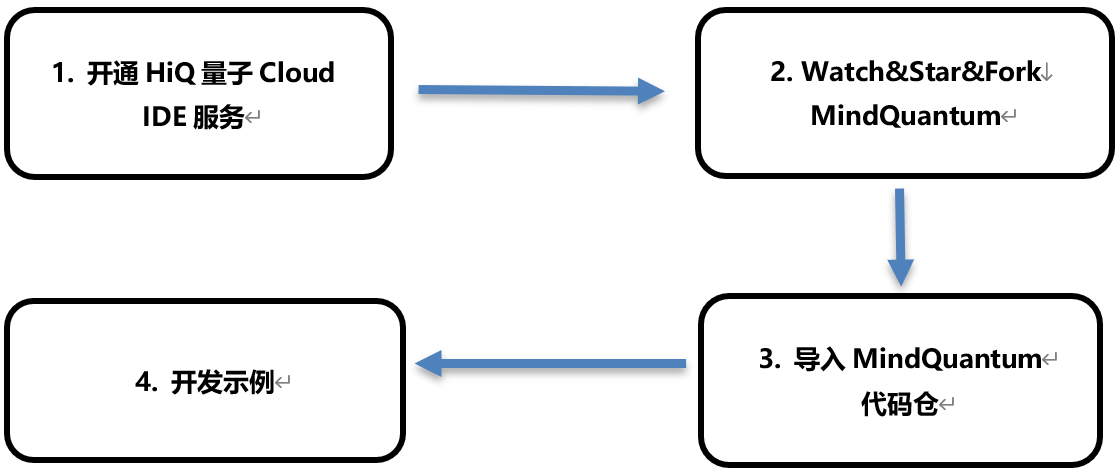
\includegraphics[width=0.5\linewidth]{1.png} % 插入svg出了点问题
%     \caption{1.svg}
%     \label{fig:enter-label}
% \end{figure}

% \end{document}
